\documentclass{extbook}[14pt]
\usepackage{multicol, enumerate, enumitem, hyperref, color, soul, setspace, parskip, fancyhdr, amssymb, amsthm, amsmath, latexsym, units, mathtools}
\everymath{\displaystyle}
\usepackage[headsep=0.5cm,headheight=0cm, left=1 in,right= 1 in,top= 1 in,bottom= 1 in]{geometry}
\usepackage{dashrule}  % Package to use the command below to create lines between items
\newcommand{\litem}[1]{\item #1

\rule{\textwidth}{0.4pt}}
\pagestyle{fancy}
\lhead{}
\chead{Answer Key for Progress Quiz 3 Version B}
\rhead{}
\lfoot{3012-8528}
\cfoot{}
\rfoot{Summer C 2021}
\begin{document}
\textbf{This key should allow you to understand why you choose the option you did (beyond just getting a question right or wrong). \href{https://xronos.clas.ufl.edu/mac1105spring2020/courseDescriptionAndMisc/Exams/LearningFromResults}{More instructions on how to use this key can be found here}.}

\textbf{If you have a suggestion to make the keys better, \href{https://forms.gle/CZkbZmPbC9XALEE88}{please fill out the short survey here}.}

\textit{Note: This key is auto-generated and may contain issues and/or errors. The keys are reviewed after each exam to ensure grading is done accurately. If there are issues (like duplicate options), they are noted in the offline gradebook. The keys are a work-in-progress to give students as many resources to improve as possible.}

\rule{\textwidth}{0.4pt}

\begin{enumerate}\litem{
Describe the end behavior of the polynomial below.
\[ f(x) = 4(x + 3)^{4}(x - 3)^{9}(x + 2)^{4}(x - 2)^{6} \]The solution is the graph below, which is option D.
    \begin{center}
        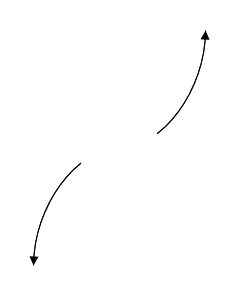
\includegraphics[width=0.3\textwidth]{../Figures/polyEndBehaviorCopyDB.png}
    \end{center}\begin{enumerate}[label=\Alph*.]
\begin{multicols}{2}
\item 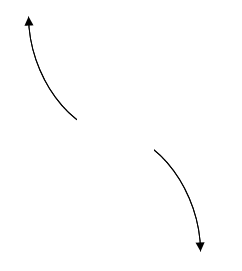
\includegraphics[width = 0.3\textwidth]{../Figures/polyEndBehaviorCopyAB.png}
\item 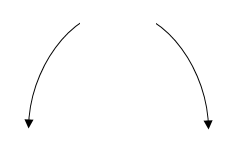
\includegraphics[width = 0.3\textwidth]{../Figures/polyEndBehaviorCopyBB.png}
\item 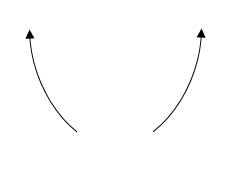
\includegraphics[width = 0.3\textwidth]{../Figures/polyEndBehaviorCopyCB.png}
\item 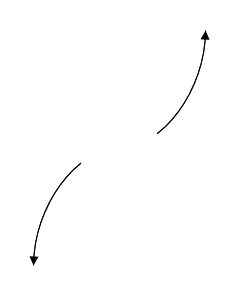
\includegraphics[width = 0.3\textwidth]{../Figures/polyEndBehaviorCopyDB.png}
\end{multicols}\item None of the above.\end{enumerate}
\textbf{General Comment:} Remember that end behavior is determined by the leading coefficient AND whether the \textbf{sum} of the multiplicities is positive or negative.
}
\litem{
Describe the zero behavior of the zero $x = -8$ of the polynomial below.
\[ f(x) = -3(x + 9)^{6}(x - 9)^{5}(x + 8)^{14}(x - 8)^{9} \]The solution is the graph below, which is option B.
    \begin{center}
        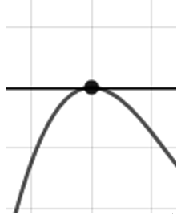
\includegraphics[width=0.3\textwidth]{../Figures/polyZeroBehaviorBB.png}
    \end{center}\begin{enumerate}[label=\Alph*.]
\begin{multicols}{2}
\item 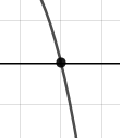
\includegraphics[width = 0.3\textwidth]{../Figures/polyZeroBehaviorAB.png}
\item 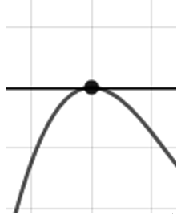
\includegraphics[width = 0.3\textwidth]{../Figures/polyZeroBehaviorBB.png}
\item 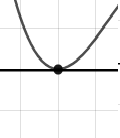
\includegraphics[width = 0.3\textwidth]{../Figures/polyZeroBehaviorCB.png}
\item 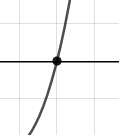
\includegraphics[width = 0.3\textwidth]{../Figures/polyZeroBehaviorDB.png}
\end{multicols}\item None of the above.\end{enumerate}
\textbf{General Comment:} You will need to sketch the entire graph, then zoom in on the zero the question asks about.
}
\litem{
Which of the following equations \textit{could} be of the graph presented below?

\begin{center}
    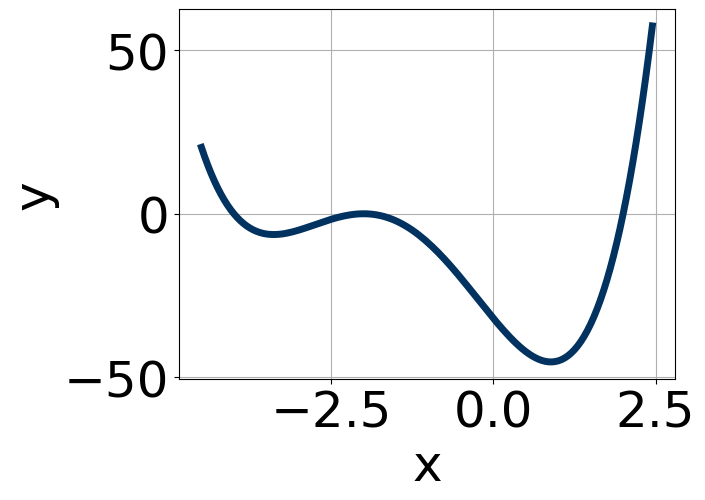
\includegraphics[width=0.5\textwidth]{../Figures/polyGraphToFunctionB.png}
\end{center}


The solution is \( 17(x + 2)^{10} (x - 2)^{7} (x + 4)^{5} \), which is option A.\begin{enumerate}[label=\Alph*.]
\item \( 17(x + 2)^{10} (x - 2)^{7} (x + 4)^{5} \)

* This is the correct option.
\item \( -9(x + 2)^{10} (x - 2)^{9} (x + 4)^{11} \)

This corresponds to the leading coefficient being the opposite value than it should be.
\item \( -18(x + 2)^{10} (x - 2)^{11} (x + 4)^{10} \)

The factor $(x + 4)$ should have an odd power and the leading coefficient should be the opposite sign.
\item \( 8(x + 2)^{7} (x - 2)^{4} (x + 4)^{5} \)

The factor $-2$ should have an even power and the factor $2$ should have an odd power.
\item \( 20(x + 2)^{4} (x - 2)^{4} (x + 4)^{9} \)

The factor $(x - 2)$ should have an odd power.
\end{enumerate}

\textbf{General Comment:} General Comments: Draw the x-axis to determine which zeros are touching (and so have even multiplicity) or cross (and have odd multiplicity).
}
\litem{
Construct the lowest-degree polynomial given the zeros below. Then, choose the intervals that contain the coefficients of the polynomial in the form $x^3+bx^2+cx+d$.
\[ 3 + 2 i \text{ and } 4 \]The solution is \( x^{3} -10 x^{2} +37 x -52 \), which is option C.\begin{enumerate}[label=\Alph*.]
\item \( b \in [1, 8], c \in [-7.52, -6.31], \text{ and } d \in [11, 13] \)

$x^{3} + x^{2} -7 x + 12$, which corresponds to multiplying out $(x -3)(x -4)$.
\item \( b \in [5, 14], c \in [36.76, 37.91], \text{ and } d \in [49, 57] \)

$x^{3} +10 x^{2} +37 x + 52$, which corresponds to multiplying out $(x-(3 + 2 i))(x-(3 - 2 i))(x + 4)$.
\item \( b \in [-15, -7], c \in [36.76, 37.91], \text{ and } d \in [-52, -48] \)

* $x^{3} -10 x^{2} +37 x -52$, which is the correct option.
\item \( b \in [1, 8], c \in [-6.57, -5.83], \text{ and } d \in [6, 9] \)

$x^{3} + x^{2} -6 x + 8$, which corresponds to multiplying out $(x -2)(x -4)$.
\item \( \text{None of the above.} \)

This corresponds to making an unanticipated error or not understanding how to use nonreal complex numbers to create the lowest-degree polynomial. If you chose this and are not sure what you did wrong, please contact the coordinator for help.
\end{enumerate}

\textbf{General Comment:} Remember that the conjugate of $a+bi$ is $a-bi$. Since these zeros always come in pairs, we need to multiply out $(x-(3 + 2 i))(x-(3 - 2 i))(x-(4))$.
}
\litem{
Which of the following equations \textit{could} be of the graph presented below?

\begin{center}
    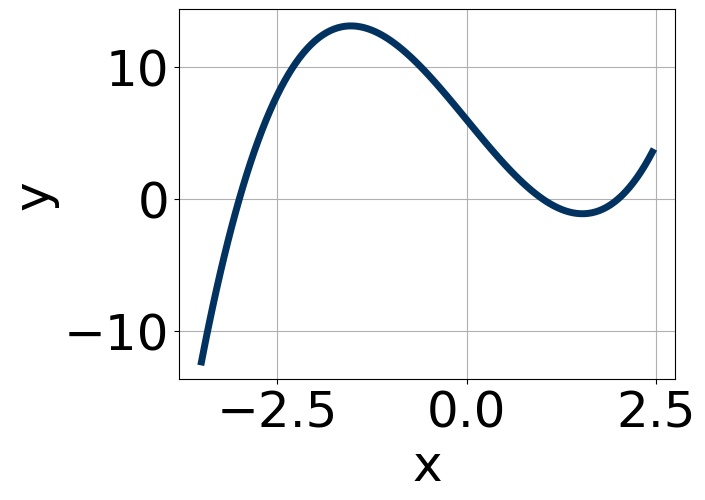
\includegraphics[width=0.5\textwidth]{../Figures/polyGraphToFunctionCopyB.png}
\end{center}


The solution is \( 16(x - 2)^{5} (x + 3)^{5} (x - 1)^{5} \), which is option B.\begin{enumerate}[label=\Alph*.]
\item \( 4(x - 2)^{4} (x + 3)^{6} (x - 1)^{5} \)

The factors $2$ and $-3$ have have been odd power.
\item \( 16(x - 2)^{5} (x + 3)^{5} (x - 1)^{5} \)

* This is the correct option.
\item \( -9(x - 2)^{10} (x + 3)^{9} (x - 1)^{7} \)

The factor $(x - 2)$ should have an odd power and the leading coefficient should be the opposite sign.
\item \( 4(x - 2)^{6} (x + 3)^{7} (x - 1)^{11} \)

The factor $2$ should have been an odd power.
\item \( -10(x - 2)^{11} (x + 3)^{5} (x - 1)^{7} \)

This corresponds to the leading coefficient being the opposite value than it should be.
\end{enumerate}

\textbf{General Comment:} General Comments: Draw the x-axis to determine which zeros are touching (and so have even multiplicity) or cross (and have odd multiplicity).
}
\litem{
Describe the end behavior of the polynomial below.
\[ f(x) = -9(x + 8)^{4}(x - 8)^{5}(x - 6)^{4}(x + 6)^{5} \]The solution is the graph below, which is option B.
    \begin{center}
        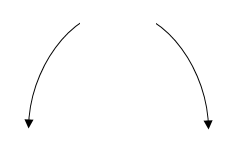
\includegraphics[width=0.3\textwidth]{../Figures/polyEndBehaviorBB.png}
    \end{center}\begin{enumerate}[label=\Alph*.]
\begin{multicols}{2}
\item 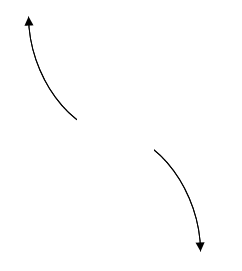
\includegraphics[width = 0.3\textwidth]{../Figures/polyEndBehaviorAB.png}
\item 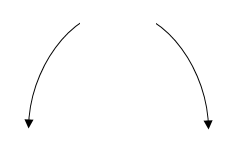
\includegraphics[width = 0.3\textwidth]{../Figures/polyEndBehaviorBB.png}
\item 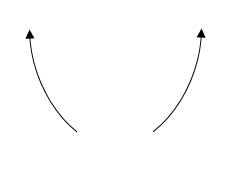
\includegraphics[width = 0.3\textwidth]{../Figures/polyEndBehaviorCB.png}
\item 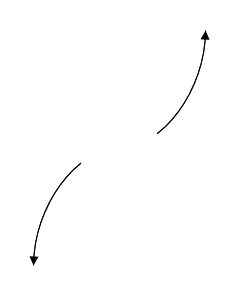
\includegraphics[width = 0.3\textwidth]{../Figures/polyEndBehaviorDB.png}
\end{multicols}\item None of the above.\end{enumerate}
\textbf{General Comment:} Remember that end behavior is determined by the leading coefficient AND whether the \textbf{sum} of the multiplicities is positive or negative.
}
\litem{
Describe the zero behavior of the zero $x = -5$ of the polynomial below.
\[ f(x) = -9(x - 5)^{4}(x + 5)^{7}(x - 9)^{4}(x + 9)^{8} \]The solution is the graph below, which is option A.
    \begin{center}
        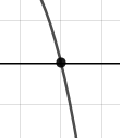
\includegraphics[width=0.3\textwidth]{../Figures/polyZeroBehaviorCopyAB.png}
    \end{center}\begin{enumerate}[label=\Alph*.]
\begin{multicols}{2}
\item 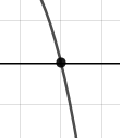
\includegraphics[width = 0.3\textwidth]{../Figures/polyZeroBehaviorCopyAB.png}
\item 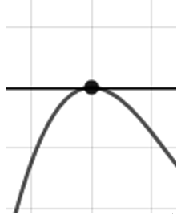
\includegraphics[width = 0.3\textwidth]{../Figures/polyZeroBehaviorCopyBB.png}
\item 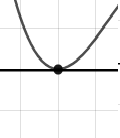
\includegraphics[width = 0.3\textwidth]{../Figures/polyZeroBehaviorCopyCB.png}
\item 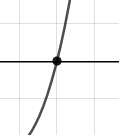
\includegraphics[width = 0.3\textwidth]{../Figures/polyZeroBehaviorCopyDB.png}
\end{multicols}\item None of the above.\end{enumerate}
\textbf{General Comment:} You will need to sketch the entire graph, then zoom in on the zero the question asks about.
}
\litem{
Construct the lowest-degree polynomial given the zeros below. Then, choose the intervals that contain the coefficients of the polynomial in the form $ax^3+bx^2+cx+d$.
\[ 1, \frac{-3}{4}, \text{ and } \frac{6}{5} \]The solution is \( 20x^{3} -29 x^{2} -9 x + 18 \), which is option A.\begin{enumerate}[label=\Alph*.]
\item \( a \in [20, 21], b \in [-35, -25], c \in [-9, 1], \text{ and } d \in [15, 24] \)

* $20x^{3} -29 x^{2} -9 x + 18$, which is the correct option.
\item \( a \in [20, 21], b \in [-22, -14], c \in [-21, -16], \text{ and } d \in [15, 24] \)

$20x^{3} -19 x^{2} -21 x + 18$, which corresponds to multiplying out $(x + 1)(4x -3)(5x -6)$.
\item \( a \in [20, 21], b \in [27, 36], c \in [-9, 1], \text{ and } d \in [-26, -17] \)

$20x^{3} +29 x^{2} -9 x -18$, which corresponds to multiplying out $(x + 1)(4x -3)(5x + 6)$.
\item \( a \in [20, 21], b \in [-35, -25], c \in [-9, 1], \text{ and } d \in [-26, -17] \)

$20x^{3} -29 x^{2} -9 x -18$, which corresponds to multiplying everything correctly except the constant term.
\item \( a \in [20, 21], b \in [10, 12], c \in [-33, -25], \text{ and } d \in [-26, -17] \)

$20x^{3} +11 x^{2} -27 x -18$, which corresponds to multiplying out $(x + 1)(4x + 3)(5x -6)$.
\end{enumerate}

\textbf{General Comment:} To construct the lowest-degree polynomial, you want to multiply out $(x -1)(4x + 3)(5x -6)$
}
\litem{
Construct the lowest-degree polynomial given the zeros below. Then, choose the intervals that contain the coefficients of the polynomial in the form $x^3+bx^2+cx+d$.
\[ 3 + 4 i \text{ and } 4 \]The solution is \( x^{3} -10 x^{2} +49 x -100 \), which is option D.\begin{enumerate}[label=\Alph*.]
\item \( b \in [-5, 7], c \in [-7.9, -4.2], \text{ and } d \in [11, 13] \)

$x^{3} + x^{2} -7 x + 12$, which corresponds to multiplying out $(x -3)(x -4)$.
\item \( b \in [-5, 7], c \in [-8.4, -7.9], \text{ and } d \in [13, 18] \)

$x^{3} + x^{2} -8 x + 16$, which corresponds to multiplying out $(x -4)(x -4)$.
\item \( b \in [7, 19], c \in [48.6, 51.5], \text{ and } d \in [98, 101] \)

$x^{3} +10 x^{2} +49 x + 100$, which corresponds to multiplying out $(x-(3 + 4 i))(x-(3 - 4 i))(x + 4)$.
\item \( b \in [-10, -4], c \in [48.6, 51.5], \text{ and } d \in [-102, -94] \)

* $x^{3} -10 x^{2} +49 x -100$, which is the correct option.
\item \( \text{None of the above.} \)

This corresponds to making an unanticipated error or not understanding how to use nonreal complex numbers to create the lowest-degree polynomial. If you chose this and are not sure what you did wrong, please contact the coordinator for help.
\end{enumerate}

\textbf{General Comment:} Remember that the conjugate of $a+bi$ is $a-bi$. Since these zeros always come in pairs, we need to multiply out $(x-(3 + 4 i))(x-(3 - 4 i))(x-(4))$.
}
\litem{
Construct the lowest-degree polynomial given the zeros below. Then, choose the intervals that contain the coefficients of the polynomial in the form $ax^3+bx^2+cx+d$.
\[ \frac{3}{4}, \frac{5}{2}, \text{ and } -4 \]The solution is \( 8x^{3} +6 x^{2} -89 x + 60 \), which is option C.\begin{enumerate}[label=\Alph*.]
\item \( a \in [5, 9], b \in [16, 29], c \in [-71, -68], \text{ and } d \in [-63, -58] \)

$8x^{3} +18 x^{2} -71 x -60$, which corresponds to multiplying out $(4x + 3)(2x -5)(x + 4)$.
\item \( a \in [5, 9], b \in [-13, -5], c \in [-95, -76], \text{ and } d \in [-63, -58] \)

$8x^{3} -6 x^{2} -89 x -60$, which corresponds to multiplying out $(4x + 3)(2x + 5)(x -4)$.
\item \( a \in [5, 9], b \in [2, 9], c \in [-95, -76], \text{ and } d \in [55, 66] \)

* $8x^{3} +6 x^{2} -89 x + 60$, which is the correct option.
\item \( a \in [5, 9], b \in [2, 9], c \in [-95, -76], \text{ and } d \in [-63, -58] \)

$8x^{3} +6 x^{2} -89 x -60$, which corresponds to multiplying everything correctly except the constant term.
\item \( a \in [5, 9], b \in [57, 64], c \in [115, 125], \text{ and } d \in [55, 66] \)

$8x^{3} +58 x^{2} +119 x + 60$, which corresponds to multiplying out $(4x + 3)(2x + 5)(x + 4)$.
\end{enumerate}

\textbf{General Comment:} To construct the lowest-degree polynomial, you want to multiply out $(4x -3)(2x -5)(x + 4)$
}
\end{enumerate}

\end{document}